
%% bare_conf.tex
%% V1.4b
%% 2015/08/26
%% by Michael Shell
%% See:
%% http://www.michaelshell.org/
%% for current contact information.
%%
%% This is a skeleton file demonstrating the use of IEEEtran.cls
%% (requires IEEEtran.cls version 1.8b or later) with an IEEE
%% conference paper.
%%
%% Support sites:
%% http://www.michaelshell.org/tex/ieeetran/
%% http://www.ctan.org/pkg/ieeetran
%% and
%% http://www.ieee.org/

%%*************************************************************************
%% Legal Notice:
%% This code is offered as-is without any warranty either expressed or
%% implied; without even the implied warranty of MERCHANTABILITY or
%% FITNESS FOR A PARTICULAR PURPOSE! 
%% User assumes all risk.
%% In no event shall the IEEE or any contributor to this code be liable for
%% any damages or losses, including, but not limited to, incidental,
%% consequential, or any other damages, resulting from the use or misuse
%% of any information contained here.
%%
%% All comments are the opinions of their respective authors and are not
%% necessarily endorsed by the IEEE.
%%
%% This work is distributed under the LaTeX Project Public License (LPPL)
%% ( http://www.latex-project.org/ ) version 1.3, and may be freely used,
%% distributed and modified. A copy of the LPPL, version 1.3, is included
%% in the base LaTeX documentation of all distributions of LaTeX released
%% 2003/12/01 or later.
%% Retain all contribution notices and credits.
%% ** Modified files should be clearly indicated as such, including  **
%% ** renaming them and changing author support contact information. **
%%*************************************************************************


% *** Authors should verify (and, if needed, correct) their LaTeX system  ***
% *** with the testflow diagnostic prior to trusting their LaTeX platform ***
% *** with production work. The IEEE's font choices and paper sizes can   ***
% *** trigger bugs that do not appear when using other class files.       ***                          ***
% The testflow support page is at:
% http://www.michaelshell.org/tex/testflow/



\documentclass[conference]{IEEEtran}
% Some Computer Society conferences also require the compsoc mode option,
% but others use the standard conference format.
%
% If IEEEtran.cls has not been installed into the LaTeX system files,
% manually specify the path to it like:
% \documentclass[conference]{../sty/IEEEtran}





% Some very useful LaTeX packages include:
% (uncomment the ones you want to load)


% *** MISC UTILITY PACKAGES ***
%
%\usepackage{ifpdf}
% Heiko Oberdiek's ifpdf.sty is very useful if you need conditional
% compilation based on whether the output is pdf or dvi.
% usage:
% \ifpdf
%   % pdf code
% \else
%   % dvi code
% \fi
% The latest version of ifpdf.sty can be obtained from:
% http://www.ctan.org/pkg/ifpdf
% Also, note that IEEEtran.cls V1.7 and later provides a builtin
% \ifCLASSINFOpdf conditional that works the same way.
% When switching from latex to pdflatex and vice-versa, the compiler may
% have to be run twice to clear warning/error messages.






% *** CITATION PACKAGES ***
%
%\usepackage{cite}
% cite.sty was written by Donald Arseneau
% V1.6 and later of IEEEtran pre-defines the format of the cite.sty package
% \cite{} output to follow that of the IEEE. Loading the cite package will
% result in citation numbers being automatically sorted and properly
% "compressed/ranged". e.g., [1], [9], [2], [7], [5], [6] without using
% cite.sty will become [1], [2], [5]--[7], [9] using cite.sty. cite.sty's
% \cite will automatically add leading space, if needed. Use cite.sty's
% noadjust option (cite.sty V3.8 and later) if you want to turn this off
% such as if a citation ever needs to be enclosed in parenthesis.
% cite.sty is already installed on most LaTeX systems. Be sure and use
% version 5.0 (2009-03-20) and later if using hyperref.sty.
% The latest version can be obtained at:
% http://www.ctan.org/pkg/cite
% The documentation is contained in the cite.sty file itself.
\usepackage{graphicx}

\usepackage{enumitem}
\usepackage{multicol,lipsum}



% *** GRAPHICS RELATED PACKAGES ***
%
\ifCLASSINFOpdf
  % \usepackage[pdftex]{graphicx}
  % declare the path(s) where your graphic files are
  % \graphicspath{{../pdf/}{../jpeg/}}
  % and their extensions so you won't have to specify these with
  % every instance of \includegraphics
  % \DeclareGraphicsExtensions{.pdf,.jpeg,.png}
\else
  % or other class option (dvipsone, dvipdf, if not using dvips). graphicx
  % will default to the driver specified in the system graphics.cfg if no
  % driver is specified.
  % \usepackage[dvips]{graphicx}
  % declare the path(s) where your graphic files are
  % \graphicspath{{../eps/}}
  % and their extensions so you won't have to specify these with
  % every instance of \includegraphics
  % \DeclareGraphicsExtensions{.eps}
\fi
% graphicx was written by David Carlisle and Sebastian Rahtz. It is
% required if you want graphics, photos, etc. graphicx.sty is already
% installed on most LaTeX systems. The latest version and documentation
% can be obtained at: 
% http://www.ctan.org/pkg/graphicx
% Another good source of documentation is "Using Imported Graphics in
% LaTeX2e" by Keith Reckdahl which can be found at:
% http://www.ctan.org/pkg/epslatex
%
% latex, and pdflatex in dvi mode, support graphics in encapsulated
% postscript (.eps) format. pdflatex in pdf mode supports graphics
% in .pdf, .jpeg, .png and .mps (metapost) formats. Users should ensure
% that all non-photo figures use a vector format (.eps, .pdf, .mps) and
% not a bitmapped formats (.jpeg, .png). The IEEE frowns on bitmapped formats
% which can result in "jaggedy"/blurry rendering of lines and letters as
% well as large increases in file sizes.
%
% You can find documentation about the pdfTeX application at:
% http://www.tug.org/applications/pdftex





% *** MATH PACKAGES ***
%
%\usepackage{amsmath}
% A popular package from the American Mathematical Society that provides
% many useful and powerful commands for dealing with mathematics.
%
% Note that the amsmath package sets \interdisplaylinepenalty to 10000
% thus preventing page breaks from occurring within multiline equations. Use:
%\interdisplaylinepenalty=2500
% after loading amsmath to restore such page breaks as IEEEtran.cls normally
% does. amsmath.sty is already installed on most LaTeX systems. The latest
% version and documentation can be obtained at:
% http://www.ctan.org/pkg/amsmath





% *** SPECIALIZED LIST PACKAGES ***
%
%\usepackage{algorithmic}
% algorithmic.sty was written by Peter Williams and Rogerio Brito.
% This package provides an algorithmic environment fo describing algorithms.
% You can use the algorithmic environment in-text or within a figure
% environment to provide for a floating algorithm. Do NOT use the algorithm
% floating environment provided by algorithm.sty (by the same authors) or
% algorithm2e.sty (by Christophe Fiorio) as the IEEE does not use dedicated
% algorithm float types and packages that provide these will not provide
% correct IEEE style captions. The latest version and documentation of
% algorithmic.sty can be obtained at:
% http://www.ctan.org/pkg/algorithms
% Also of interest may be the (relatively newer and more customizable)
% algorithmicx.sty package by Szasz Janos:
% http://www.ctan.org/pkg/algorithmicx




% *** ALIGNMENT PACKAGES ***
%
%\usepackage{array}
% Frank Mittelbach's and David Carlisle's array.sty patches and improves
% the standard LaTeX2e array and tabular environments to provide better
% appearance and additional user controls. As the default LaTeX2e table
% generation code is lacking to the point of almost being broken with
% respect to the quality of the end results, all users are strongly
% advised to use an enhanced (at the very least that provided by array.sty)
% set of table tools. array.sty is already installed on most systems. The
% latest version and documentation can be obtained at:
% http://www.ctan.org/pkg/array


% IEEEtran contains the IEEEeqnarray family of commands that can be used to
% generate multiline equations as well as matrices, tables, etc., of high
% quality.




% *** SUBFIGURE PACKAGES ***
%\ifCLASSOPTIONcompsoc
%  \usepackage[caption=false,font=normalsize,labelfont=sf,textfont=sf]{subfig}
%\else
%  \usepackage[caption=false,font=footnotesize]{subfig}
%\fi
% subfig.sty, written by Steven Douglas Cochran, is the modern replacement
% for subfigure.sty, the latter of which is no longer maintained and is
% incompatible with some LaTeX packages including fixltx2e. However,
% subfig.sty requires and automatically loads Axel Sommerfeldt's caption.sty
% which will override IEEEtran.cls' handling of captions and this will result
% in non-IEEE style figure/table captions. To prevent this problem, be sure
% and invoke subfig.sty's "caption=false" package option (available since
% subfig.sty version 1.3, 2005/06/28) as this is will preserve IEEEtran.cls
% handling of captions.
% Note that the Computer Society format requires a larger sans serif font
% than the serif footnote size font used in traditional IEEE formatting
% and thus the need to invoke different subfig.sty package options depending
% on whether compsoc mode has been enabled.
%
% The latest version and documentation of subfig.sty can be obtained at:
% http://www.ctan.org/pkg/subfig




% *** FLOAT PACKAGES ***
%
%\usepackage{fixltx2e}
% fixltx2e, the successor to the earlier fix2col.sty, was written by
% Frank Mittelbach and David Carlisle. This package corrects a few problems
% in the LaTeX2e kernel, the most notable of which is that in current
% LaTeX2e releases, the ordering of single and double column floats is not
% guaranteed to be preserved. Thus, an unpatched LaTeX2e can allow a
% single column figure to be placed prior to an earlier double column
% figure.
% Be aware that LaTeX2e kernels dated 2015 and later have fixltx2e.sty's
% corrections already built into the system in which case a warning will
% be issued if an attempt is made to load fixltx2e.sty as it is no longer
% needed.
% The latest version and documentation can be found at:
% http://www.ctan.org/pkg/fixltx2e


%\usepackage{stfloats}
% stfloats.sty was written by Sigitas Tolusis. This package gives LaTeX2e
% the ability to do double column floats at the bottom of the page as well
% as the top. (e.g., "\begin{figure*}[!b]" is not normally possible in
% LaTeX2e). It also provides a command:
%\fnbelowfloat
% to enable the placement of footnotes below bottom floats (the standard
% LaTeX2e kernel puts them above bottom floats). This is an invasive package
% which rewrites many portions of the LaTeX2e float routines. It may not work
% with other packages that modify the LaTeX2e float routines. The latest
% version and documentation can be obtained at:
% http://www.ctan.org/pkg/stfloats
% Do not use the stfloats baselinefloat ability as the IEEE does not allow
% \baselineskip to stretch. Authors submitting work to the IEEE should note
% that the IEEE rarely uses double column equations and that authors should try
% to avoid such use. Do not be tempted to use the cuted.sty or midfloat.sty
% packages (also by Sigitas Tolusis) as the IEEE does not format its papers in
% such ways.
% Do not attempt to use stfloats with fixltx2e as they are incompatible.
% Instead, use Morten Hogholm'a dblfloatfix which combines the features
% of both fixltx2e and stfloats:
%
% \usepackage{dblfloatfix}
% The latest version can be found at:
% http://www.ctan.org/pkg/dblfloatfix




% *** PDF, URL AND HYPERLINK PACKAGES ***
%
%\usepackage{url}
% url.sty was written by Donald Arseneau. It provides better support for
% handling and breaking URLs. url.sty is already installed on most LaTeX
% systems. The latest version and documentation can be obtained at:
% http://www.ctan.org/pkg/url
% Basically, \url{my_url_here}.




% *** Do not adjust lengths that control margins, column widths, etc. ***
% *** Do not use packages that alter fonts (such as pslatex).         ***
% There should be no need to do such things with IEEEtran.cls V1.6 and later.
% (Unless specifically asked to do so by the journal or conference you plan
% to submit to, of course. )


% correct bad hyphenation here
\hyphenation{op-tical net-works semi-conduc-tor}


\begin{document}
%
% paper title
% Titles are generally capitalized except for words such as a, an, and, as,
% at, but, by, for, in, nor, of, on, or, the, to and up, which are usually
% not capitalized unless they are the first or last word of the title.
% Linebreaks \\ can be used within to get better formatting as desired.
% Do not put math or special symbols in the title.
\title{Multi Layer Perceptron - Project 3}


% author names and affiliations
% use a multiple column layout for up to three different
% affiliations
\author{\IEEEauthorblockN{Madhusudan Govindraju	}
\IEEEauthorblockA{
University of Florida\\
Email: madhusudangr@ufl.edu}
}

% conference papers do not typically use \thanks and this command
% is locked out in conference mode. If really needed, such as for
% the acknowledgment of grants, issue a \IEEEoverridecommandlockouts
% after \documentclass

% for over three affiliations, or if they all won't fit within the width
% of the page, use this alternative format:
% 
%\author{\IEEEauthorblockN{Michael Shell\IEEEauthorrefmark{1},
%Homer Simpson\IEEEauthorrefmark{2},
%James Kirk\IEEEauthorrefmark{3}, 
%Montgomery Scott\IEEEauthorrefmark{3} and
%Eldon Tyrell\IEEEauthorrefmark{4}}
%\IEEEauthorblockA{\IEEEauthorrefmark{1}School of Electrical and Computer Engineering\\
%Georgia Institute of Technology,
%Atlanta, Georgia 30332--0250\\ Email: see http://www.michaelshell.org/contact.html}
%\IEEEauthorblockA{\IEEEauthorrefmark{2}Twentieth Century Fox, Springfield, USA\\
%Email: homer@thesimpsons.com}
%\IEEEauthorblockA{\IEEEauthorrefmark{3}Starfleet Academy, San Francisco, California 96678-2391\\
%Telephone: (800) 555--1212, Fax: (888) 555--1212}
%\IEEEauthorblockA{\IEEEauthorrefmark{4}Tyrell Inc., 123 Replicant Street, Los Angeles, California 90210--4321}}




% use for special paper notices
%\IEEEspecialpapernotice{(Invited Paper)}




% make the title area
\maketitle

% As a general rule, do not put math, special symbols or citations
% in the abstract
\begin{abstract}
This paper gives an introduction to multi layer perceptron and how it works. Analyses the results of a multi layer perceptron. Finally the paper gives an idea on how to construct multi layer perceptron for recognizing handwritten digits with the MNIST dataset. The paper will include assumptions and procedures taken to achieve at the parameters and the structure of the network. The multi layer perceptron uses a set of processing elements to form layers in a neural network. The structure of the neural network depends on the application for which it is being used. An activation function is the final step in the processing unit. The activation function turns the output of the processing element on or off based on the input. The level (or value) of the output depends on the activation function being used.

\end{abstract}


\begin{IEEEkeywords} 
Rosenblatt's Perceptron, Perceptron, Adaline, Multi Layer Perceptron (MLP), Stochastic gradient descent
\end{IEEEkeywords}

% no keywords




% For peer review papers, you can put extra information on the cover
% page as needed:
% \ifCLASSOPTIONpeerreview
% \begin{center} \bfseries EDICS Category: 3-BBND \end{center}
% \fi
%
% For peerreview papers, this IEEEtran command inserts a page break and
% creates the second title. It will be ignored for other modes.
\IEEEpeerreviewmaketitle



\section{Introduction}

\begin{figure}[h!]
\centering
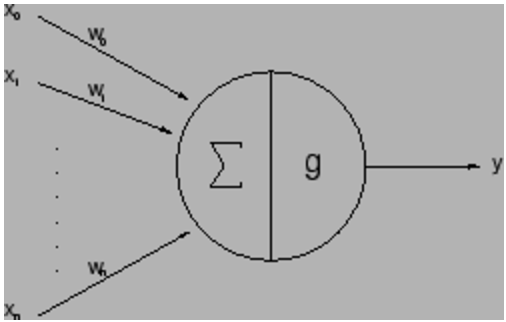
\includegraphics[scale=0.5]{neuron}
\caption{A Structure of a Neuron}
\label{neuron}
\end{figure}

\begin{figure}[h!]
\centering
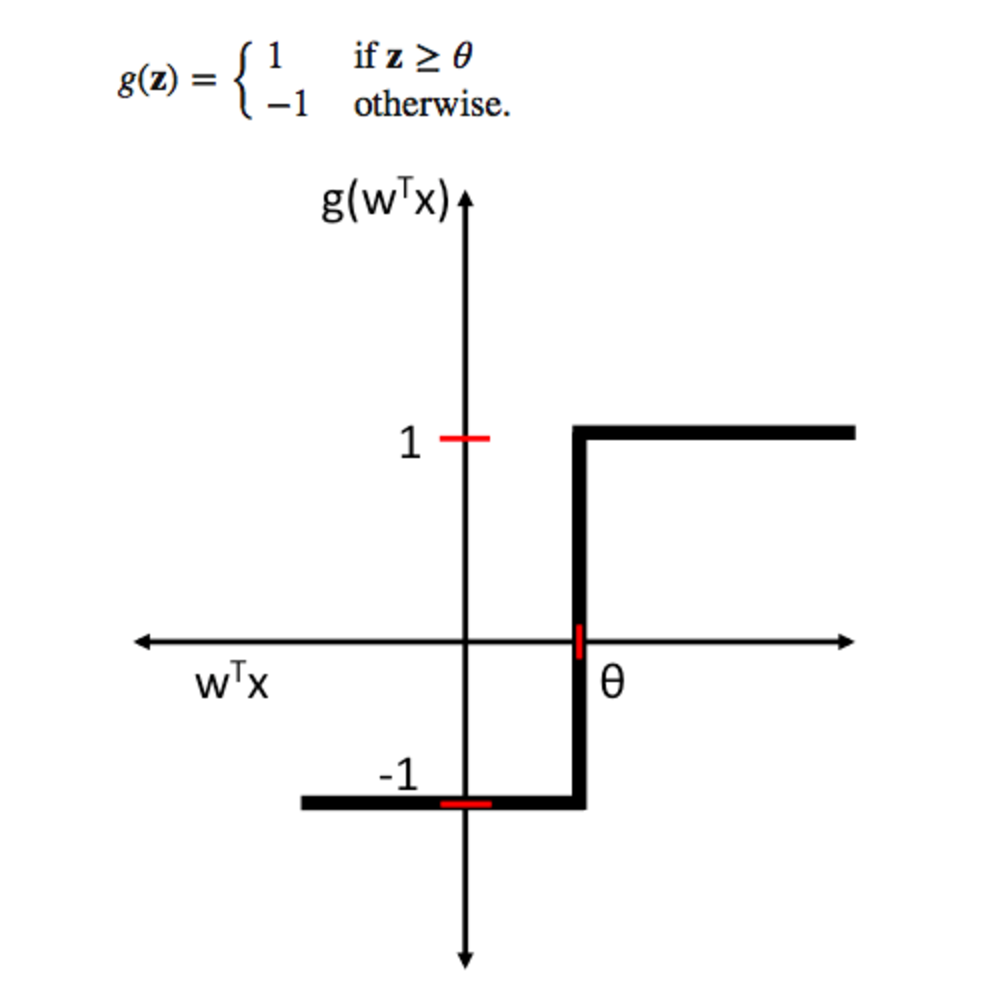
\includegraphics[scale=0.25]{threshold_activation}
\caption{Threshold Activation Function}
\label{threshold}
\end{figure}

\begin{figure}[h!]
\centering
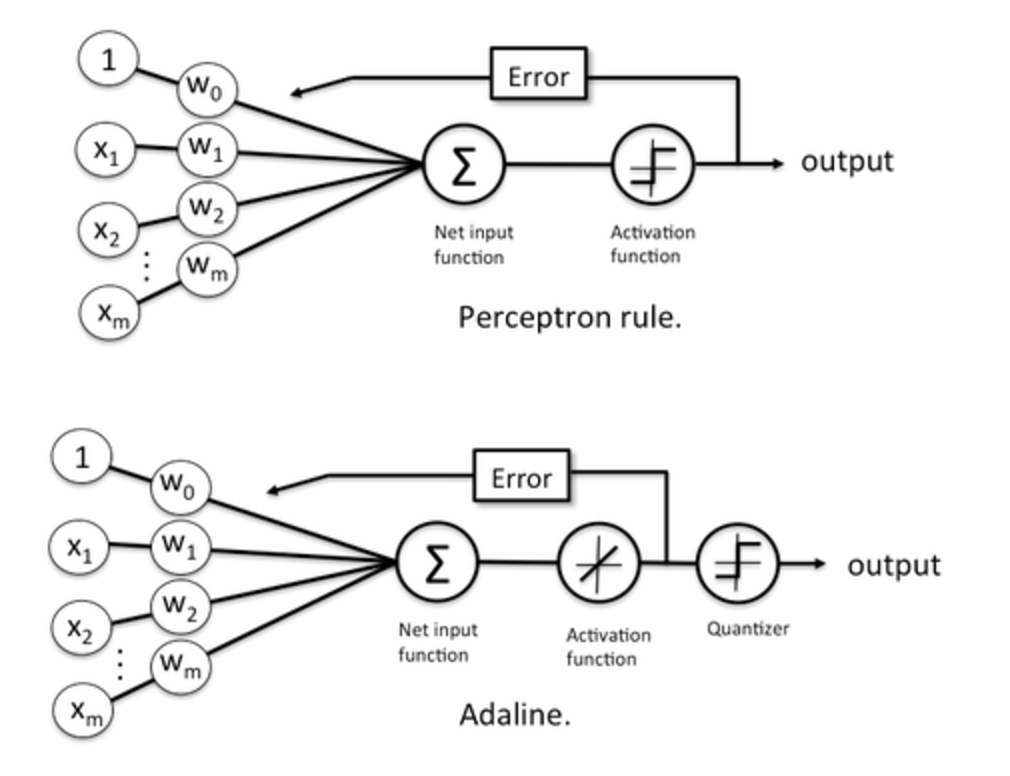
\includegraphics[scale=0.5]{Adaline_Perceptron}
\caption{The Adaline and Perceptron Model - here real activation function in the Adaline is actually the quantizer but for comparison purposes (with perceptron model) the units are named as Activation function \& Quantizer }
\label{Adaline Perceptron}
\end{figure}


The multi layer perceptrons are made up of multiple processing elements the structure of a processing element is shown in the figure \ref{neuron}. In this figure \ref{neuron} 'g' is the activation function. The processing elements of a multi layer perceptron has been built upon the Perceptron model and Adaline as a basis\cite{RosenBlat's Perceptron} \cite{Marlyn Neural Nets} \cite{Gail Neural Nets}. They both have the same structure of a processing element in a multi layer perceptron. These models use threshold function as an activation function, hence the outputs(net) of each element is linear. An example of the threshold activation function is available in the figure \ref{threshold}. There are a few differences between the perceptron and the Adaline model. The perceptron uses the linear activation function to give as input to the feedback unit. While in the Adaline model we use an non linear activation function in the training phase to give as an input to the feedback unit, with the final output is still quantized by an linear threshold activation function. We can also refer to the Adaline as the stochastic gradient descent model. The perceptron can also be referred to as the  Rosenblatt?s Perceptron model.

 \begin{figure}[h!]
\centering
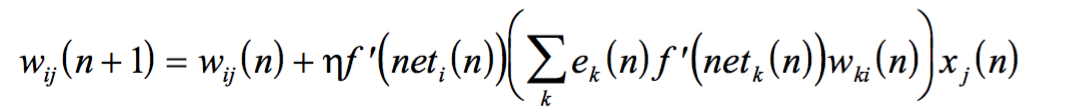
\includegraphics[scale=0.45]{backpropogation}
\caption{The equation to update the weights in the back-propagation algorithm}
\label{backpropagation}
\end{figure}

The learning algorithm is a gradient descent technique. Here the optimization problem is to reduce the cost(error) of the system. The algorithm is devised in such a way that the error trickles down to all the processing elements and their respective weights are corrected. Just as in a normal gradient descent algorithm even this algorithm has a constant to control the learning rate. The general equation to change the weighs in a layer is given by the equation in the figure \ref{backpropagation} 
 
 \begin{figure}[h!]
\centering
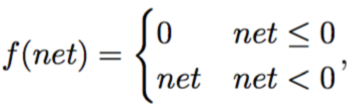
\includegraphics[scale=0.5]{RELU}
\caption{Rectified Linear Activation Function, ReLU }

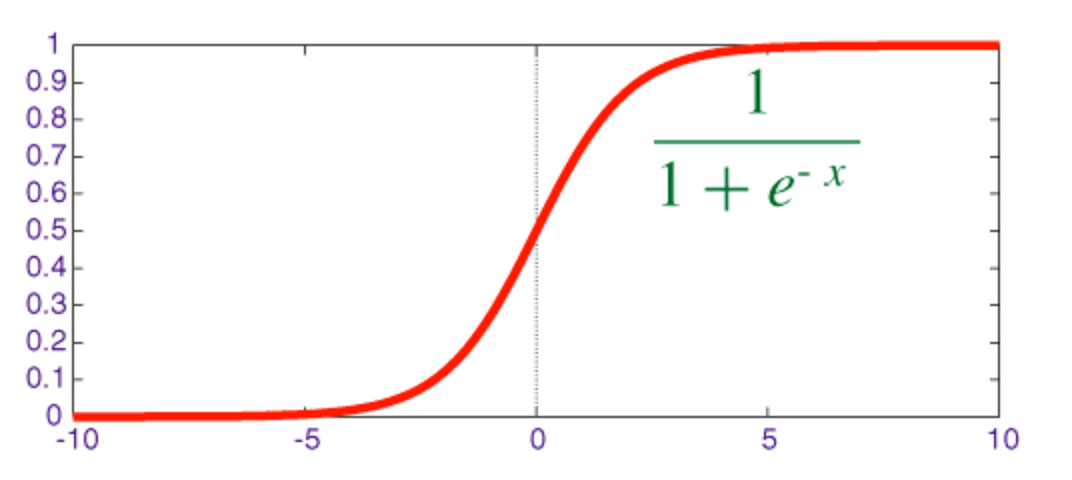
\includegraphics[scale=0.45]{sigmoid}
\caption{Sigmoid Activation Function}

\label{relu}
\end{figure}
 
The multi layer perceptrons use a layer (or multiple layers) of perceptrons except for the fact that they use a non linear activation function such as the hyperbolic sigmoid, hyperbolic tangent function or rectified linear unit activation function(ReLU). In our project we will be using the rectified linear activation function (fig \ref{relu}). The advantage of using a sigmoid function over a step function is that they are differentiable. 
 
 \begin{figure}[h!]
\centering
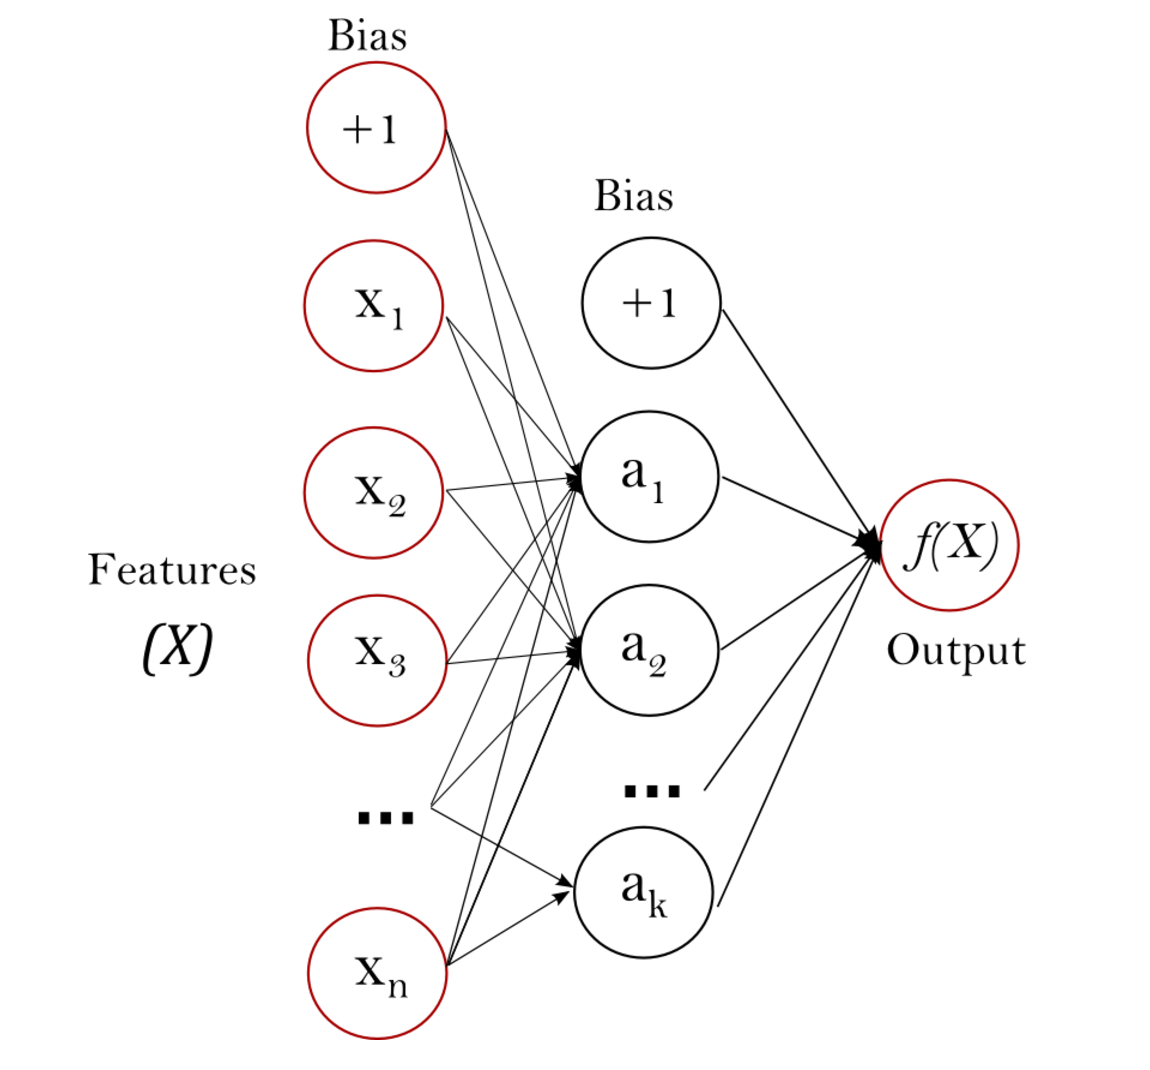
\includegraphics[scale=0.45]{MLP}
\caption{Multi Layer Perceptron \cite{MLPfigure}}
\label{MLP}
\end{figure}
 
The basic structure of an MLP is shown in figure \ref{MLP}.  

The most common algorithm used to train MLP is the back propogation algorithm and it consists of two steps: feed forward, in this step the data is run through the network and the network's output is calcualted; the second step back propagation, in this step error for processing element in every hidden is calculated and their respective weights are adjusted throughout the network. To update the weights we use the delta rule(chain rule of partial derivatives). As we use label/information from the data set to train the network this is classified under supervised learning.


\section{The Data}

\begin{figure}[h!]
\centering
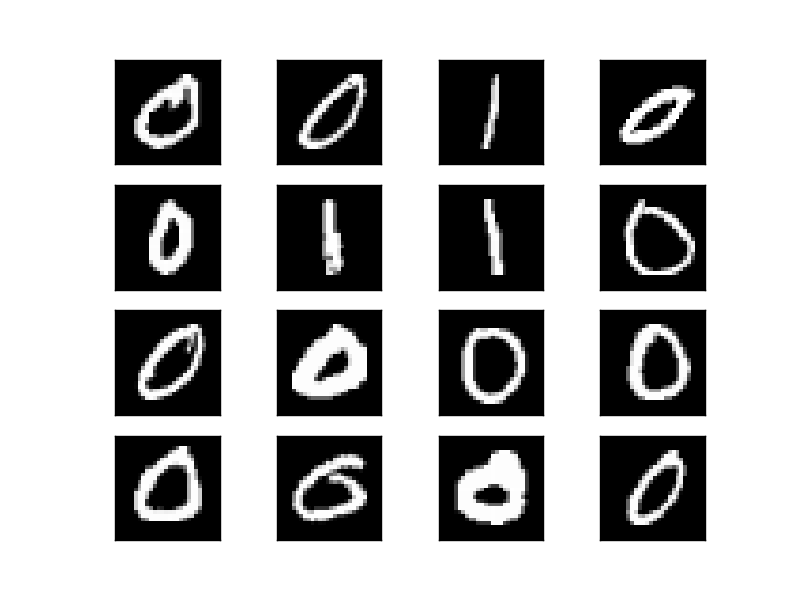
\includegraphics[scale=0.45]{Inputsample.png}
\caption{Sample images of the handwritten digits from the dataset}
\label{input}
\end{figure}

\begin{table}[]
\centering
\caption{Data Set Ratio}
\label{dataset ratio}
\begin{tabular}{|l|l|l|l|}
\hline
                                                              & \begin{tabular}[c]{@{}l@{}}Test\\ Set\end{tabular} & \begin{tabular}[c]{@{}l@{}}Training\\ Set\end{tabular} & \begin{tabular}[c]{@{}l@{}}Validation\\ Set\end{tabular} \\ \hline
\begin{tabular}[c]{@{}l@{}}Number\\ of\\ Samples\end{tabular} & 10K                                                & 50K                                                    & 10K                                                      \\ \hline
\end{tabular}
\end{table}


This paper uses the MNIST \cite{MNIST} dataset for implementing a multi layer perceptron. The dataset consists of 70,000 images each with dimension of 784(28x28 image), with pixel intensities as the contents of the vector. These pixel intensities are in the grayscale range with intensities ranging from zero to 255.  Some of the images from the dataset are available in the figure \ref{input}. MNIST is a dataset of handwritten digits.

From the figure \ref{input} we can see that the digits are towards the center an the pixels towards the edges have no significant value. These pixels can be avoided by applying an dimensionality reduction algorithm such as PCA to the dataset before feeding it into the network. The other thing that is evident from the images is that the digits are towards the center and some pixels will not align perfectly with the others from the same class hence matching just using the pixel intensities is not going to give us much accuracy. For this we need to look into methods that use only the most discriminating features from the dataset. This is again a PCA problem and can be solved by applying PCA to the dataset before training or testing on it. The MNIST dataset is of the most studied dataset in the machine learning branch. Thus it is commonly used to rank a machine learning algorithm.

The database consists of 70,000 images. We perform random sampling and the first 50000 images are taken as training images , 50,000-60,000 images is taken as validation set and the 60,000 -70,000 are taken as test set. If we don't do random sampling we will loose data, such as the first 60,000 images in the dataset dont have any class 9 images, hence while testing the class 9 images will all be predicted along with the other classes. 
Random sampling also increases the generality of the system. In case the database has all the classes in order, the system learns(optimizes weights) better for the first class (example class 0) and then when a class 1 object is presented the system juts labels it as a second class rather than finding a way to differentiate the class, this is what happened in the first configuration shown in the appendix. 

\section{Implementation and Evaluation of the Network}
\subsection{Mini-Batch Size}
This neural network makes use of a varient of gradient descent technique to arrive at the optimal weights. It uses the entire batch of input data before updating the weights, also referred to as a batch update. In our case we use stochastic gradient descent algorithm to achieve convergence. In this method we use a mini batch to achieve the convergence much sooner also by using a mini-batch with random sampling we can omit problems of the dataset such as preordering of all samples of the same class together. This increases the generalization of the network. The size of the mini batch varies with application, the best was to achieve at the mini batch size is to do a grid search, but for our case we can run the algorithm multiple number of times with a few set of values for min batch and ball park at a figure. In our case the number of samples in each class(in training set) is approximately 5000, hence choosing a value close to 10,000 is going to have at-least 2 classes (worst case scenario) in 1 loop and hence in one epoch(for entire training set) we would have a good generalization. Hence we ballpark at a mini batch size of 10,000 for our further steps. Also keeping a very small batch size the number of epochs needed to arrive at the optimal point is very large.

\subsection{Processign Elements}
Since we know that using one, two, three, and four processing elements in the hidden layer gives us one decision boundary, two separate decision boundaries, enclosed decision boundary and disjoint boundaries respectively. We can understand that the number of processing elements in the hidden layer for our case is going to be more than 4. 

Since the digits we are trying to classify are more complex than the cases mentioned above, we are starting one hidden layer with 50 processing elements in the hidden layer. The input layer is the same size of the input that is 784. (The input image of 28x28 is stretched out into one vector of size 784). The output layer is going to have processing elements 10(softmax), one for each class. We get a meagre 26 \% accuracy for the test data for 30 epochs. The dataset seems to converge quickly hence we are using just 30 epochs for training. More information about this step can be seen in the learning rate graph shown in figure \ref{50HL}

Now we will run the same network with 250 processing elements in the hidden layer, we get the same accuracy of 82\%. This suggests that just increasing the number of processing elements in the hidden layer generally increases the accuracy of the network. Similarly for 500 processing elements in the hidden later we get an accuracy of 89\%. Increasing the number of processing elements increases the time to train the system as well as gives a better accuracy. From the table \ref{processing Elements} we can also infer that after a certain point the number of hidden layer elements does not make the network better, while we were able to achieve better performance by increasing the number of hidden layers in the network from one to two. This gave us 98\% accuracy. 

Here the performance of the network has been gauged by its accuracy. The table \ref{processing Elements} gives us an idea of how the accuracy varies with different number of processing elements. Clearly as mentioned above the number of processing elements increase the accuracy increases only till a limit, but after that the increase is very little or none, this can be seen (in table \ref{processing Elements}) when using 250 and 500 elements in the same hidden layer of the network. On increasing the number of hidden layers the accuracy again increases. More details are available in the confusion matrices in the appendix and  figures \ref{all PE} and \ref{50HL}.

\begin{table}[]
\centering
\caption{Accuracy of the N/w for varying number of Processing Elements and PCA}
\label{processing Elements}
\begin{tabular}{|l|l|l|}
\hline
\begin{tabular}[c]{@{}l@{}}No. Hidden \\ Layer PE\end{tabular} & \begin{tabular}[c]{@{}l@{}}Accuracy\\ w/o PCA\end{tabular} & \begin{tabular}[c]{@{}l@{}}Accuracy\\ with PCA\end{tabular} \\ \hline
50                                                             & 26                                                         & N/A                                                         \\ \hline
250                                                            & 82                                                         & 92                                                          \\ \hline
500                                                            & 89                                                         & 95                                                          \\ \hline
1000, 100                                                      & 98                                                         & 98                                                          \\ \hline
\end{tabular}
\end{table}


\begin{figure}[h!]
\centering
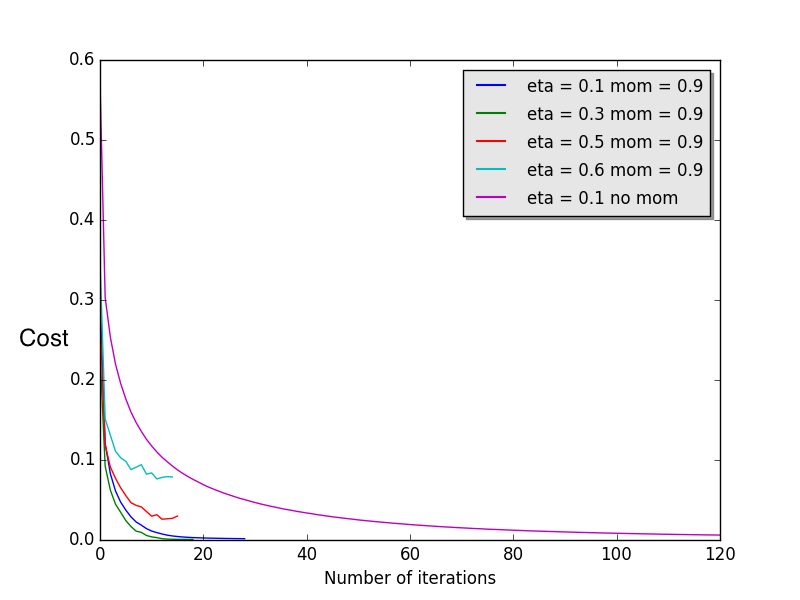
\includegraphics[scale=0.45]{learningRate.png}
\caption{Learning Rate vs Learning Curve}
\label{learning rate vs learning curve graph}
\footnotesize{This graph shows how the learning varies with different learning rates. The learning rates 0.6 and 0.5 do not converge or converge at sub optimal positions, while 03 and 0.1 converge at optimal points and 0.1 is more smooth. The learning with and without momentum is also depicted here}
\end{figure}



\subsection{Learning Rate}
For the stochastic gradient descent the learning rate is much smaller than the normal batch update gradient descent algorithm. We continuously validate the network against a validation dataset and update the learning rate after every epoch (or after few epochs). This gives better convergence. We check for values ranging from 0.1 to 1 and see that we get the best convergence at 0.1. We choose learning rate at 0.1 for our further procedures.The easiest way to achieve an optimal learning rate is to choose a suitable constant small value for learning rate such that it gives a stable \& smooth convergence.  The other reason why we have a smaller learning rate is to complement the high momentum given to the network.

\begin{figure}[h!]
\centering
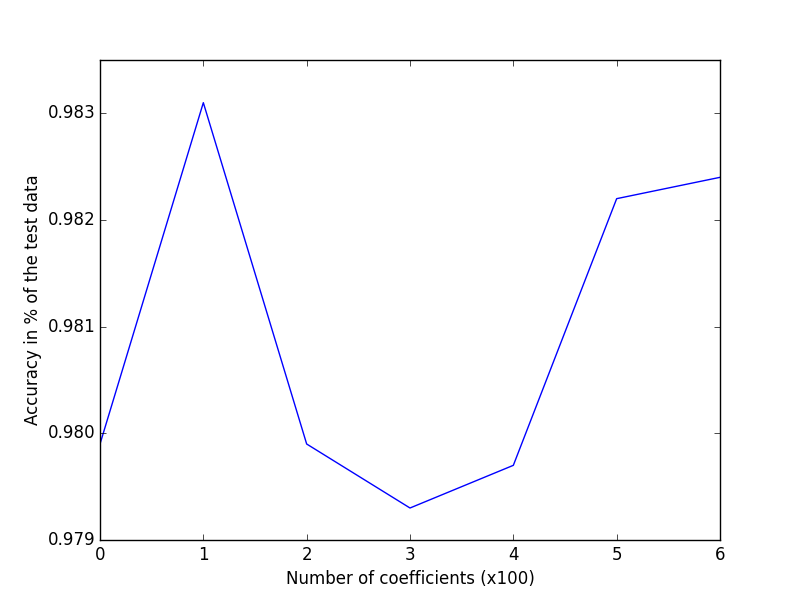
\includegraphics[scale=0.45]{pca100.png}
\caption{PCA vs Accuracy}
\label{pca100}
\footnotesize{The change in accuracy is very less (approx 0.2\% variance), but we get the best performance for top 100 coefficients, hence proving that it is not required to use all 784 pixels for this dataset. The network configurations used were 250 processing elements in hidden layers, 1e-4 regularization constant.}
\end{figure}

\subsection{PCA}

In the next step we try to apply a feature reduction algorithm to remove the redundant pixels in the images which are not required for classification. By applying the PCA to the dataset and taking only 100 best features of the 784 features  from the dataset. The performance increases to 88.40\% for 500 processing elements. This gives us an idea that there are a lot of pixel intensities that are not required for classification and can be omitted during the process. A solution for this is provided in \cite{Google Nets}. The table \ref{processing Elements} gives us this detail. From the confusion matrices 5,6\&7 available in the appendix we can clearly see that one class is not classified properly with just 500 or 250 processing elements. This effect of using direct pixel intensities can be ignored if using a very large network (confusion matrix 8 , case 4: 1000,100 hidden layer) .



\subsection{Activation Function}
\begin{figure}[h!]
\centering
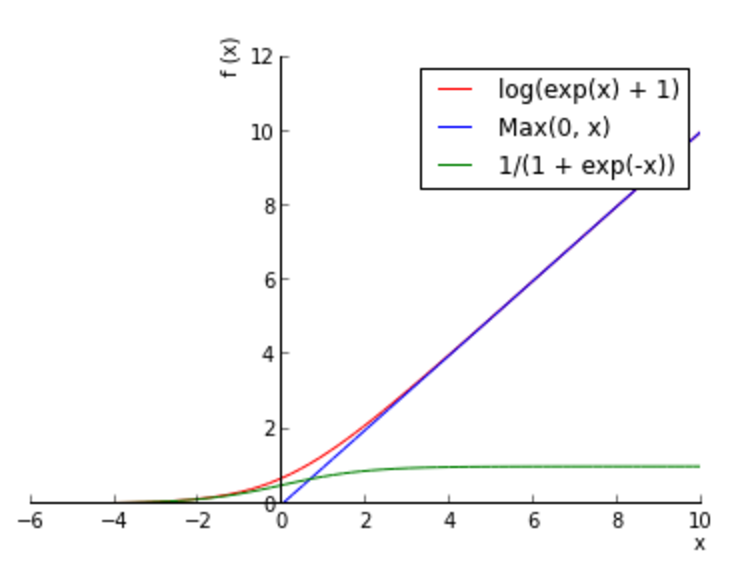
\includegraphics[scale=0.5]{relucomparison}
\caption{Comparison of ReLU with sigmoid and tanH}
\label{relu comparison}
\footnotesize{Here the Max(0,x) is the ReLU function, log(exp(x)+1) is the hyperbolic tangent and 1/(1+e(-x)) is the sigmoid function. With the increase in the x(in our case this is the output of the PE), the sigmoid has almost zero slope when closer to the one and zero, while hyperbolic tangent has almost zero slope initial cases when the error is close to zero, but for ReLU the value is directly proportional to the x(so slope is greater or never=0 until the error is zero).}
\end{figure}
Generally we use hyperbolic tangent and the log functions for gradient descent in back propagation algorithms because the derivative can be calculated as a function of the processing element's output, for tanh it is $1 - u^2$ and for the logistic function it is $u * (1 - u)$. While \cite{relu} \& \cite{relu why faster} say that rectified linear unit(ReLU) is six times faster than the hyperbolic tangent function. In our case using ReLU or hyperbolic tangent gives us very less difference. This is explained in the figure \ref{relu comparison} and the comparisons of different activation function for our network is available in figure \ref{Activation Function}.

The sigmoid function or the logistic function will be more appropriate in cases where we try to model probabilities. while ReLU can used in cases where we need to model positive numbers. In our case we are trying to predict the classes which are real numbers and hence ReLU will be a better choice. This leas us to understand that even the labels we are trying to predict has a small impact on the structure of the neural network we are trying to build. In case we use one hot encoding and provide the class labels as [1,0,0,0,0,0,0,0,0,0] for class 0 and [0,1,0,0,0,0,0,0,0,0] for class 1 and so on hyperbolic tangent should perform better, but checking this beyond the scope of this report and not verified here.

 Hence with the figure \ref{relu comparison} we prove that ReLU does not have the vanishing gradient problem (sigmoid and tanh are prone to this), and thus provides earlier convergence. and we use that in the other experiments that follow in this report.


\subsection{Momentum}

\begin{figure}[h!]
\centering
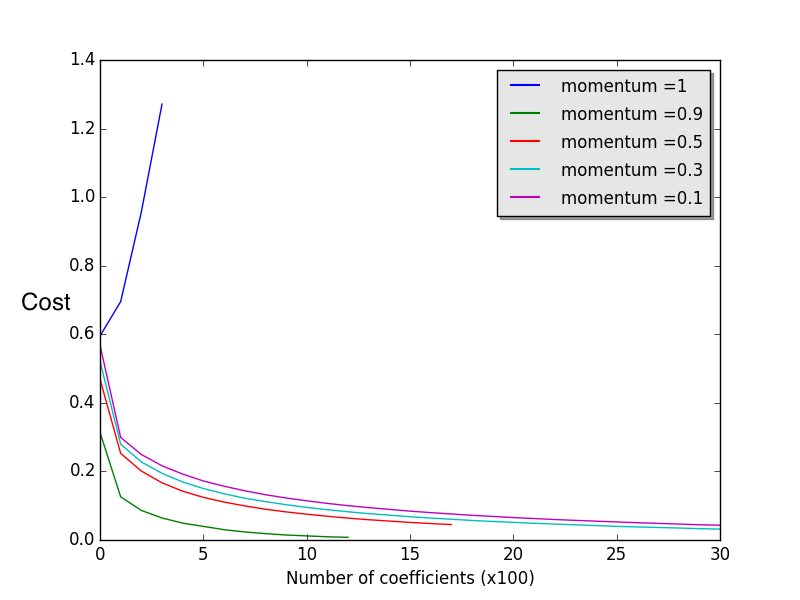
\includegraphics[scale=0.45]{momentumVsAccuracy.png}
\caption{Momentum vs Learning Curve}
\label{momVSacc}
\footnotesize{This graph depicts how the learning curve varies with the different momentum constants. We get the best performance at 0.9 and the least at 1. For a momentum 1 according to rule the learning stops the earliest, but the learning does not converge, this is the case where the gradient descent passes over the local minima. The accuracies for these curves are available in table \ref{momTable}. The network configurations used were 250 processing elements in hidden layer, 1e-4 regularization constant, ReLU activation function, and learning rate eta of 0.1.}
\end{figure}

We have previously seen that gradient descent will find the local optimum/minimum and not the global optimum. And that is because the local minimum is much closer to the starting point. There are ways to get over this problem, but we cannot say for a certain that the minimum we obtained is global minimum. One way is to run the network with different starting weights and check if the optimum obtained is local or global. This is highly computationally expensive and we might not arrive at the global solution at all. Another method is to give a momentum to the gradient descent algorithm so that, the gradient will help us jump over the shallow minimum and into the steeper minimum. Thus we are able to achieve a higher accuracy for the same dataset, with the a lesser number of processing elements. The confusion matrices and their respective accuracies are available in 9,10,11,12,13  in the \textbf{Results} section , table \ref{momTable},  figure \ref{momVSacc}, figure \ref{all PE} compare systems with different momentum values. 

\begin{figure}[h!]
\centering
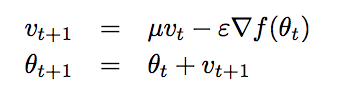
\includegraphics[scale=1]{momentum}
\caption{Stochastic Gradient Descent - momentum update \cite{momentum} }
\footnotesize{Here $\epsilon$ is the learning rate and should be greater than 0, $\mu$ is the momentum and should be between 0 and 1}
\label{Momentum_eq}
\end{figure}

\begin{table}[]
\centering
\caption{Momentum vs Accuracy}
\label{momTable}
\begin{tabular}{|l|l|}
\hline
\begin{tabular}[c]{@{}l@{}}Momentum\\ Constant\end{tabular} & \begin{tabular}[c]{@{}l@{}}Accuracy\\ w/o PCA\end{tabular} \\ \hline
0.1                                                         & 98                                                         \\ \hline
0.3                                                         & 97                                                         \\ \hline
0.5                                                         & 98                                                         \\ \hline
0.9                                                         & 98                                                         \\ \hline
1                                                           & 82                                                         \\ \hline
\end{tabular}
\end{table}

The equation for updating the gradient descent's momentum is available in the figure \ref{Momentum_eq}. The momentum function adds a fraction of the previous weight to the current weight, so if the gradient keeps changing direction it will smooth out the directions and help achieve the optimal point in lesser iterations. This complements the low learning rate we are using in the network, as the momentum used is 0.9 we are limiting our learning rate to 0.1.




\subsection{Regularization}
\begin{figure}[h!]
\centering
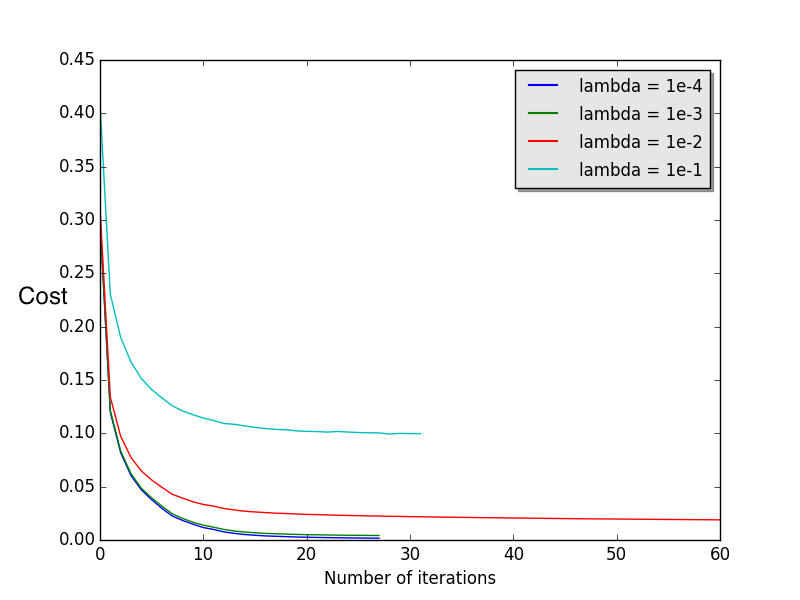
\includegraphics[scale=0.45]{regularizationVSlearningCurve.png}
\caption{Regularization Const vs Learning Curve }
\label{regularization graph}
\end{figure}


From the above mentioned cases we can see that the training accuracy is almost 100\% this means the network has been memorized the training set. .We should apply some generalization technique to make sure the algorithm does not overfit or memorize the training data. This is almost impossible in the case of neural network because we are using large numbers of hidden layer processing elements. If we have more parameters(weights) in the system compared to the number of features in the sample set, we will definitely overfit the training data. 
\begin{itemize}
\item \textbf{L2 Regularization term:} Applying L2 regularization term is another method of preventing overfitting the data, but still since the number of processing elements is huge in this case, we cant help overfitting the training data and hence other generalization measures should also be applied. This L2 regularization penalizes large weights 
\item \textbf{Randomizing Initial weights:} Each back propagation training algorithm starts with different initial weights and biases and hence arriving at different solutions each time we run the algorithm. Hence its bet practice to run the network multiple number of times are choose the one which gives the best performance. This process will help in generalization. 
\item \textbf{Early Stop:} Another method is the early stop method. In this method we continuously check for the error of the validation set. When the network begins to memorize the training set, the error of the validation set will rise. This will be the right time to stop training the network. (figure \ref{Early Stop})
\end{itemize}

Instead of implementing a grid search for the L2 regularization parameter we use heuristic methods to ball park at a good L2 regularization parameter. The cost obtained for for different L2 parameters are given in detail in the appendix. The different L2 parameters used are 1(default/initial condition), $1e^{-4}$,$1e^{-3}$ \&$0.1$. We find that we get the best performance for $1e^{-4}$. (figure \ref{regularization graph})

Reasons for choosing the above mentioned L2 parameters: we can see than the learning curve is not smooth for the system with no regularization parameter, there is a sudden initial drop in the learning curve, hence we need a very small regularization parameter value to stop the initial drop of the learning curve of the un-regularized system. Hence obtaining a much smoother learning curve. Smooth learning curve results in better generalization of the training data. 

\subsection{Dropout}

\begin{figure}[h!]
\centering
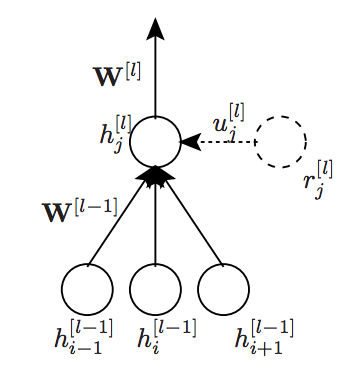
\includegraphics[height=2in]{dropout}
\caption{An illustration of dropout \cite{dropout}}
\label{dropout fig}
\end{figure}

In all the above mentioned cases the training set performance in the network yeilded perfect 100\% accuracy. This means that we have overfitted the network, even though we have applied regularization terms, we get a near perfect accuracy or perfect confusion matrix for the training dataset (refer to confusion matrix in result 14 in \textbf{Results} section). Dropout is a technique where we add a stochastic processing element to a normal processing element in the hidden layer of a network \cite{dropout}. An illustration for dropout is available in figure \ref{dropout fig}. The activation function with a dropout changes to 

\begin{figure}[h!]
\centering
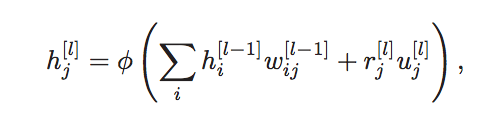
\includegraphics[scale=0.5]{dropoutEquation}
%\caption{An illustration of dropout \cite{dropout}}
%\label{dropout fig}
\end{figure}
where $h_{i}^{l-1}$ $w_{ij}^{l-1}$ is the $i$-th hidden layer neuron in the $(l-1)$th hidden layer and the edge weight between $h_{i}^{l-1}$\&$h_{j}^{l}$ and $\sigma$ is any nonlinear activation function. The confusion matrix obtained by using a dropout in the network shows near 100\% accuracy(not 100\%) hence making the network more generalized, in our toy MNIST dataset, using the test dataset gives us 98\% accuracy easily but that would not be possible in real scenarios. The two confusion matrices for training dataset with and without dropout are available in the 14th and 15 result in \textbf{Results} section. We can see that even with the accuracy of the training set dropping to 99\% we achieve an 98\% accuracy as the other case without dropout implemented, again proving that dropout increases the performance of the system 







\begin{table*}[]
\caption{Complete List of Configurations and their Comparisons}
\label{complete evaluation}
\begin{tabular}{llllllllllll}
\hline
                                                        & \begin{tabular}[c]{@{}l@{}}Without\\ PCA\end{tabular} & \begin{tabular}[c]{@{}l@{}}With\\ PCA\end{tabular} & \begin{tabular}[c]{@{}l@{}}Activation\\ Function\\ (ReLU)\end{tabular} & \begin{tabular}[c]{@{}l@{}}Activation\\ Function\\ (TanH)\end{tabular} & \begin{tabular}[c]{@{}l@{}}Activation\\ Function\\ (Sigmoid)\end{tabular} & \begin{tabular}[c]{@{}l@{}}Learning\\ Rate\\ (Worst)\\ eta = \$0.6\end{tabular} & \begin{tabular}[c]{@{}l@{}}Learning\\ Rate\\ (Best)\\ eta = 0.1\end{tabular} & \begin{tabular}[c]{@{}l@{}}(Worst)\\ lambda = 0.1\end{tabular} & \begin{tabular}[c]{@{}l@{}}(Best)\\ lamda = 1e-4\end{tabular} & \begin{tabular}[c]{@{}l@{}}Momentum\\ (Worst)\\  M =0\end{tabular} & \begin{tabular}[c]{@{}l@{}}Momentum\\ (Best)\\ M=0.9\end{tabular} \\
\hline
\begin{tabular}[c]{@{}l@{}}Accuracy\\ (\%)\end{tabular} & 82                                                    & 92                                                 & 98.12                                                                  & 98.10                                                                  & 97.99                                                                     & 96.15                                                                           & 98.02                                                                        & 96.85                                                          & 98.12                                                         & 92                                                                 & 98                                                                \\
\hline
\\
Iterations                                              & 120                                                   & 120                                                & 30                                                                     & 36                                                                     & 93                                                                        & 11                                                                              & 30                                                                           & 32                                                             & 30                                                            & 120                                                                & 12                                                               \\ \hline
\end{tabular}
\footnotesize{  \\
The best configuration is , Hidden Layer 250 , ReLU Activation Function, Learning Rate - 0.1 Regularization factor = 0.1, with momentum of 0.9 and no Early Stop. Every column was populated by keeping the others columns with the above mentioned configuration, except for the PCA columns which were populated without momentum(normal SGD). This table gives us an overview of the network's performance for the different configurations. ReL U activation function converges faster than the others. The system with PCA has more accuracy for the same 250 units in hidden layer. Learning with SGDwithMomentum converges way faster compared to the others.  }

\end{table*}



\section{Conclusion}
\begin{enumerate}
\item The confusion matrices for all the above mentioned configurations are available in the \textbf{Results} section.
\item One of the issues observed with MLP is the long time it takes in the training phase. The convergence and the learning time is the main issue, if the regularization parameters are not chosen properly. 
\item Increasing the number of hidden layer elements increases the accuracy of the network
\item Using more processing elements increases the time taken to converge at the optimal point. The other confusion matrices show how worse the predictions are especially for the case (result 1) where we don't use any momentum and 50 Processing elements. The elements are clearly not enough to classify the digits and hence almost every one of them being classified into the one class. Result 1,2,3,4 show the increase in accuracy with the increase in the number of processing elements. (figure \ref{all PE})
\item  Pixel intensities are not the best features, a simple PCA increases the accuracy by approx10\%. By using a set of images created from the training images by shifting the pixels of the original image, as the training data \cite{Google Nets}, we will be able to overcome this effect of pixel intensity. The results 1,2,3,4 show the results of using PCA and the results 5,6,7,\&8 show the results of the network without using PCA.

The effect of using PCA is visualized in the confusion matrices in result 12 and 14. The network identifies class 2,4 and 9 more accurately with PCA. 

\item Choosing the appropriate learning rate lets the network learn the training data clearly. It eliminates the sudden drop in the MSE error during the initial learning phase thus, making the network more generalized.(figure \ref{learning rate vs learning curve graph})
%\item By applying regularization term to reduce the effect of over fitting  and using ReLU. for 500 number of PE we get 100\% accuracy in the training set this show that the system gets overfitted. This is avoided by using logistic function and a much higher regularization parameter. This happens because we have lesser data compare to the number of parameters in the system, which leads us to reduce the number of processing elements in the hidden layer. Hence fixing the number of processing elements to 250.
\item Logistic activation function takes a longer time to converge, but if we use the hyperbolic tangent or the ReLU function as the activation function the network converges to the optimal point sooner (figure \ref{Activation Function})
\item Adding the regularization factor increases the number of epochs required to converge but gives a smooth learning curve, a smooth learning curve corresponds to better generalization. The variation in accuracy with different regularization constants is available in the graph in figure \ref{regularization graph}
\item When early stop is used, the system stops when it begins to memorize the training data set. The change in accuracy is very less, but the graph which depicts the iteration to stop early is very clear and shows us in which iteration the network begins to memorize the training data. The graph in figure \ref {Early Stop} shows us the network's learning curve with early stop.
\item Comparing the stochastic gradient descent(SGD) with SGD momentum: Using momentum lets us achieve the global optimum. Without the SGD momentum factor we achieve only 92\% accuracy, on including the momentum it enables the gradient descent to travel over the local minima and find the global minima at 98\% accuracy. This enables us to use lesser processing elements and achieve better accuracy. With momentum the learning curve converges sooner than the network without momentum.
\item The confusion matrix for the best configuration is available in result 14 in the \textbf{Results} section. Almost every digit is correctly classified, very few are misclassified and that is negligible. The accuracy we get is 98\%. Which is same as the accuracy mentioned in the original paper \cite{MNIST}.  The best configuration for the network for our dataset if 250 elements in the first hidden layer, regularization constant(lambda) = 1e-4, learning rate(eta)=0.1, with momentum =0.9, with 100 best coefficients from PCA. We can notice that even when we use early stopping, the network has memorized the training data. and the accuracy for the training data is 100\%
\item Training with dropout reduces the overfitting (accuracy of training data reduces), increases the test data accuracy(same test accuracy with decrease in training data accuracy) [result 14 and 15]
\end{enumerate}

\begin{figure}
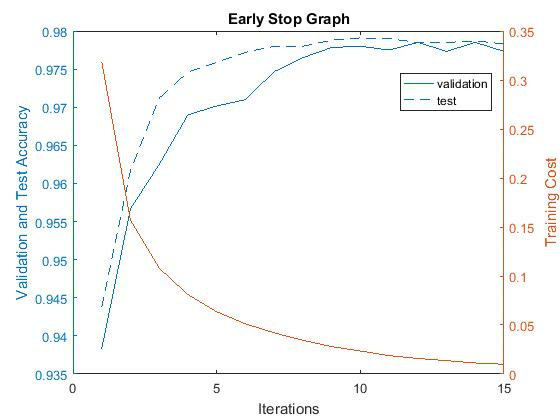
\includegraphics[scale=0.45]{EarlyStopGraph2.jpg}
\caption{Implementing Early Stop}
\footnotesize{This graph depicts one method to increase the generalization of the network. During the training of the network in each epoch we check the accuracy of the validation network,  and plotting the graph of the validation accuracy against the learning curve, we can check that after 13 iterations the accuracy of the validation set stops increasing and in-fact drops a bit hence this is the actual point where we have to stop the training iteration. After this point we can say that the network starts to memorize the training data. Hence stopping the training at iteration 13 will keep the network more generalized. \\ 
}
\label{Early Stop}
\end{figure}


\begin{figure}[h!]
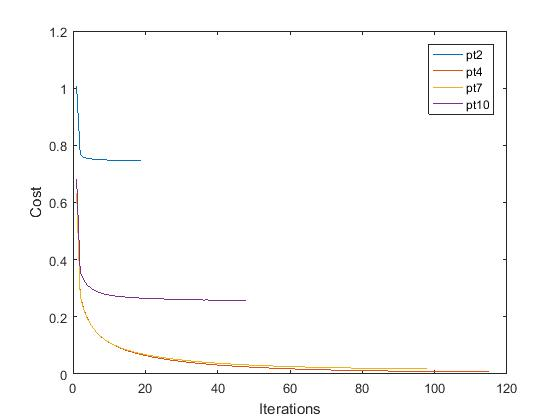
\includegraphics[scale=0.42]{hl50(1).jpg}
\caption{Learning Curve for 50 Elements in the Hidden Layer}
\footnotesize{
\textbf{Legend:} \\
pt2 = hl-50 regularization-1 logistic momentum-0.9 learningRate = 0.1\\
pt4 = hl-50 regularization-1e-4 logistic momentum-0.9 learningRate = 0.1\\
pt7 = hl-50 regularization-1e-3 logistic momentum-0.9 learningRate = 0.1\\
pt10 = hl-50 regularization-0.1 logistic momentum-0.9 learningRate = 0.1\\

From this graph, the things we can infer the following :
\begin{itemize} 
\item The Error remain too high even for the best configuration from the above
\item From this graph we can easily finalize on the regularization coefficient to 1e-4
\item Also we can tell that the error is too high and hence this 50 elements in the hidden layer is clearly not enough
\end{itemize}}
\label{50HL}
\end{figure}





\begin{figure}
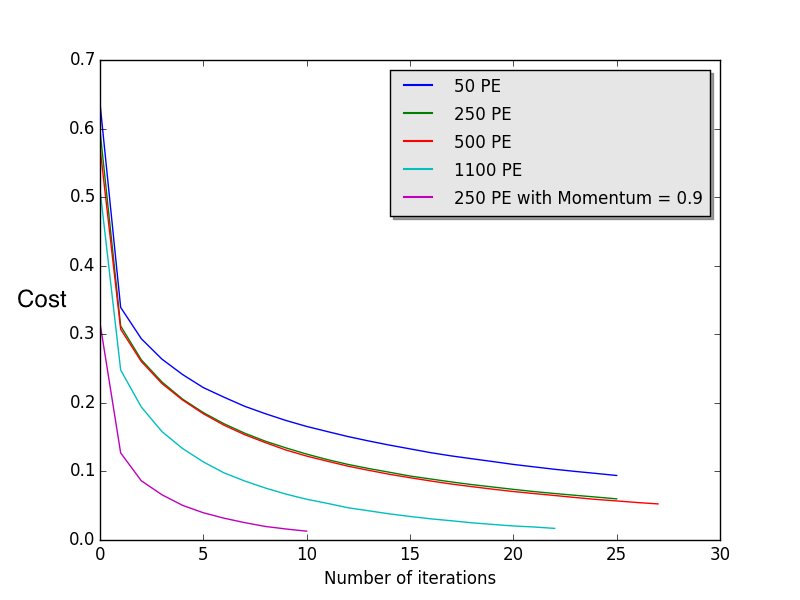
\includegraphics[scale=0.5]{PEvsAccuracy.png}
\caption{Learning Curves vs No. of Processing Elements}
\label{all PE}
\footnotesize{From the earlier graph (figure \ref{50HL})  we can clearly see that 50 hidden elements is not enough. This graph shows the performance of the network with different number of hidden layer processing elements. The higher the number of processing elements the better is the performance. But we are able to achieve that best performance with a momentum with lesser number of processing elements. From the graph we can infer the following: Large number of processing elements will increase the accuracy and take care of the irregularities in the data, but some amount of data preprocessing and adding the effect of momentum along with the general stochastic gradient descent gives us better performance with lesser number of processing elements. Lesser number of processing elements $\propto$ lesser training time $\propto$ lesser number of iterations.}
\end{figure}



\begin{figure}

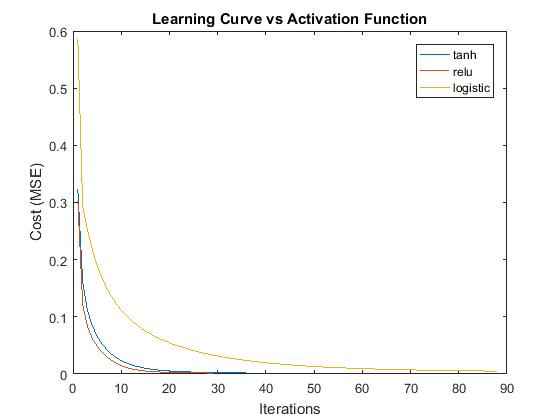
\includegraphics[scale=0.5]{activationVsLearningCurve.jpg}
\caption{Various Activation Functions for the Training Dataset}
\footnotesize{The systems different training performance for the different activation functions are mentioned in the graph above. The ReLU performs the best with the fastest convergence. The optimal point's error rate is the same for any activation function. Choosing logistic(sigmoid) activation function takes the longest to converge but if it had given a lot lesser optimal error it would have been the best. But here clearly theReLU works best. We will be using hyperbolic tangent and ReLU activation function for the other experiments in this report. }
\label{Activation Function}
\end{figure}






%\clearpage
%\newpage
\begin{thebibliography}{1}
\bibitem{MNIST}
Y. LeCun, L. Bottou, Y. Bengio, and P. Haffner. "Gradient-based learning applied to document recognition." Proceedings of the IEEE, 86(11):2278-2324, November 1998
\bibitem{RosenBlat's Perceptron}
The perceptron: A probabilistic model for information storage and organization in the brain.
Rosenblatt, F.
Psychological Review, Vol 65(6), Nov 1958, 386-408.
\bibitem{Marlyn Neural Nets}
"A Practical Guide to Neural Nets" , by Marilyn McCord Nelson
and W. T. Illingworth
\bibitem{Gail Neural Nets}
Gail A Carpenter, Neural network models for pattern recognition and associative memory, Neural Networks, Volume 2, Issue 4, 1989, Pages 243-257, ISSN 0893-6080, 
\bibitem{MLPfigure}
Figure source : $http://scikit-learn.org/stable/modules/neural_networks_supervised.html$

\bibitem{Regularization Parameter}
Frank Bauer, Mark A. Lukas, Comparingparameter choice methods for regularization of ill-posed problems, Mathematics and Computers in Simulation, Volume 81, Issue 9, May 2011, Pages 1795-1841, ISSN 0378-4754

\bibitem{Google Nets}
 Christian Szegedy and
               Wojciech Zaremba and
               Ilya Sutskever and
               Joan Bruna and
               Dumitru Erhan and
               Ian J. Goodfellow and
               Rob Fergus,
 "Intriguing properties of neural networks"


\bibitem{momentum}
On the importance of initialization and momentum in deep learning
Ilya Sutskever1
James Martens
George Dahl 
Geo?rey Hinton

\bibitem{relu}
Rectified Linear Units Improve Restricted Boltzmann Machines,. Vinod Nair ,Geoffrey E. Hinton

\bibitem{relu why faster}
ImageNet Classification with Deep Convolutional Neural Networks,. Alex Krizhevsky, Ilya Sutskever , Geoffrey E. Hinton

\bibitem{dropout}
"Understanding Dropout"., Pierre Baldi, Peter Sadowski ; Understanding Dropout:
Training Multi-Layer Perceptrons
with Auxiliary Independent Stochastic Neurons
KyungHyun Cho

\end{thebibliography}

\clearpage
\newpage
\onecolumn
\section{Results}
\begin{verbatim}
 ---------------------------------------------------------
 Checking how many processing elements (with PCA = top 100 coeffs)
 ---------------------------------------------------------
 
1)for HL = 50 , lambda = 1e-4 ; relu ; ets = 0.5 ; no momentum 
for test set:
[[   0    0    0    0    0    0    0    0    0  973]
 [   0   96    1    0    0    0    0    0    1 1048]
 [   0    0    5    0    0    6    0    0    0  999]
 [   0    0    1    1    0    1    0    0    0  976]
 [   0    1    1    0    0    1    4    0    0  951]
 [   0    0    0    3    0    9    1    0    3  870]
 [   0   12    0    0    0    1    0    0    0 1017]
 [   0    0    1    0    0    0    0    0    1 1044]
 [   0    0    0    2    0    0    2    0    3  975]
 [   0    0    0    1    0    1    7    0    0  981]] 
 accuracy = 26%

2)for HL = 250 , lambda = 1e-4 ; relu ; ets = 0.1 ; no momentum 
 For the test set:
[[ 975    0    5    0    0    5    7    1    2   14]
 [   2 1091    5   30    5    0    0    5   31    4]
 [   7    2  906   19    1    0    2   12   13    4]
 [   2    1    6  990    1   15    0    4   14   11]
 [   0    0    7    0  889    2    3    5    6   43]
 [   3    0    0   39    3  826    4    2   13   31]
 [  10    1   17    1   12   24  855    0    7    1]
 [   4    0   15   53   11    1    0  920    4   20]
 [   7    6   18   19   12   15    3   12  847   36]
 [   3    2    0   23   32    1    1   27    7  905]]
 Accuracy = 92%

3)for HL = 500 , lambda = 1e-4 ; relu ; ets = 0.1 ; no momentum    
  For the test set
[[ 996    0    3    0    2    5    4    1    5    3]
 [   0 1133    9    0    2    1    0    0   19    0]
 [   6    2  931    8    5    2    4    5   12    2]
 [   1    2   18  933    2   15    0    7   31    3]
 [   2    7    4    0  858    0    7    7    4   44]
 [   5    2    2   27    3  823   13    1   15    3]
 [   4    4    1    1   10    2  930    0    2    1]
 [  10   10   11    7    8    3    0 1011    7   14]
 [   5    5    6    7    9    8    9    1  923   11]
 [   5    2    1    4   28    8    1   23   18  891]]
 Accuracy = 95              
 \end{verbatim}
 \newpage
 \begin{verbatim}

 4)for HL = 1000,100 , lambda = 1e-4 ; relu ; ets = 0.1 ; no momentum
 For the test set
[[ 975    0    0    0    1    1    1    0    1    1]
 [   0 1128    2    0    0    0    2    2    2    0]
 [   3    1  985    5    1    0    0    3    4    2]
 [   1    0    6  981    0    8    0    5    4    1]
 [   1    3    1    0  912    0    4    1    2    8]
 [   1    0    3    3    1  907    9    2    3    4]
 [   4    0    0    0    1    2  939    0    1    0]
 [   2    2    3    1    1    0    0 1028    0    1]
 [   3    4    3    6    1    2    3    0  987    4]
 [   3    3    0    4   11    3    0    2    2  983]]
 accuracy=98%
 
 -------------------------------------------------------
 Without using PCA:
  -------------------------------------------------------
 
5)for HL = 250 , lambda = 1e-4 ; relu ; ets = 0.1 ; no momentum
 [[ 703    0    0    0    0    2    2    0    0  278]
 [   0 1006    2    0    8    1    1    1    0  119]
 [   0    2  392    1    0    0    1    9    1  597]
 [   1    0    0  701    0    7    0    3    3  316]
 [   0    0    0    0  355    0    0    0    3  643]
 [   1    0    0   11    0  383    0    1    1  480]
 [   0    0    0    0    0    1  168    0    2  805]
 [   2    0    2    1    0    1    0  831    0  184]
 [   0    1    0    1    0    0    0    0  245  729]
 [   2    0    0    3    0    0    0    7    1  979]]
 Accuracy = 90%
 
 6)for HL = 250 , lambda = 1e-4 ; relu ; ets = 0.1 ; no momentum
 [[ 618    0    0    0    0    0    0  386    0    0]
 [   0  961    5    0    7    0    0  132    0    1]
 [   0    1  610    0    0    0    1  373    1    1]
 [   0    0    3  643    0    8    0  393    0    0]
 [   0    0    0    0  210    0    0  713    0   46]
 [   2    0    0    9    0  326    2  553    9    0]
 [   0    0    3    0    0    0  286  674    1    0]
 [   1    1    2    0    4    0    0 1049    1    0]
 [   0    2    1    0    0    1    0  715  255    0]
 [   0    1    0    0    1    0    0  969    0   19]]
 Accuracy = 82%
 
 \end{verbatim}
 \newpage
 \begin{verbatim}
 
 7) for HL = 500 , lambda = 1e-4 ; relu ; ets = 0.1 ; no momentum
 For the test set
[[ 353    0    0    1    1    0    2    1    0  678]
 [   0 1004    7    1    1    1    1    2    4   82]
 [   0    6  492    5    3    0    0    4    8  475]
 [   0    2    2  536    0    3    0    2    4  467]
 [   0    0    0    0  568    2    2    2    0  416]
 [   0    1    1    0    0  363    4    0    8  479]
 [   0    0    0    0    0    3  144    0    0  844]
 [   0    1    4    0    2    2    0  782    0  249]
 [   0    2    0    0    0    0    0    0  133  837]
 [   0    2    0    1    4    1    0    0    0  995]]
 Accuracy=89%
 
8)for HL = 1000,100 , lambda = 1e-4 ; relu ; eta = 0.1 ; no momentum
 For the test set
[[1013    1    0    1    0    1    3    1    4    0]
 [   0 1134    4    3    0    0    1    1    1    0]
 [   2    0  946    3    1    1    1    4    4    2]
 [   0    0    6  998    1   11    0    0    4    3]
 [   0    1    3    0  971    0    6    0    1    7]
 [   1    0    1    6    1  895    4    0    1    1]
 [   2    2    1    0    1    3  968    0    2    0]
 [   0    4    3    1    1    1    0 1031    0    3]
 [   1    2    2    2    2    1    1    1  951    2]
 [   4    1    1    3    6    1    1    5    2  934]]
 accuracy=98%

 -----------------------------------------------------------
 With Momentum
 -----------------------------------------------------------
 
9) for HL = 250 , lambda = 1e-4 ; relu ; ets = 0.1 ; momentum = 0.1

test set:
[[ 962    0    2    0    1    1    2    2    1    0]
 [   0 1134    5    0    1    0    2    4    1    1]
 [   0    3 1002    7    4    0    1    4    4    0]
 [   0    0    8  942    0    8    0    3    6    1]
 [   2    3    1    0  968    0    3    4    2    9]
 [   1    0    1    2    0  856    4    2    6    3]
 [   6    0    2    0    2    3  973    0    0    0]
 [   0    2    5    3    5    0    0 1038    2    4]
 [   2    4    0   10    3    3    4    3  955    5]
 [   2    0    1    4    7    1    1    8    3  960]]
accuracy = 98%
\end{verbatim}
 \newpage
 \begin{verbatim}

10)for HL = 250 , lambda = 1e-4 ; relu ; ets = 0.1 ; momentum = 0.3
[[ 980    0    2    0    0    5    6    2    1    0]
 [   0 1115    7    1    0    0    1    4    2    0]
 [   3    0  983    3    1    0    1    8    1    1]
 [   0    2    3  961    0    8    0    3    9    1]
 [   2    4    2    0  917    1    4    1    1   12]
 [   3    2    2   13    1  885    9    0    1    2]
 [   3    1    1    1    1    7  960    0    0    0]
 [   0    4    6    2    5    0    1  997    1    7]
 [   6   11    2   11    2    9    2    2  915    5]
 [   3    7    1    7    9    6    0    5    0 1024]]
 accuracy=97%
 
 11)for HL = 250 , lambda = 1e-4 ; relu ; ets = 0.1 ; momentum = 0.5
 For the test set
[[ 979    1    1    1    0    3    2    0    2    2]
 [   1 1143    3    2    2    0    0    2    1    1]
 [   3    3 1030    4    0    1    5    9    5    1]
 [   0    0    6 1014    0    5    0    3    0    4]
 [   1    1    1    1  941    2    1    1    1    8]
 [   1    1    2    7    3  839    3    5    2    3]
 [   3    0    1    1    4    9  912    0    5    0]
 [   2    1    7    0    4    2    0  995    2    5]
 [   1    2    0   10    1    5    2    3  943    6]
 [   0    1    0    7    7    6    0   12    5  973]]

 12)for HL = 250 , lambda = 1e-4 ; relu ; ets = 0.1 ; momentum = 0.9
 For the test set
[[ 984    2    0    0    0    1    0    1    2    0]
 [   0 1153    4    0    3    0    3    4    3    0]
 [   4    3  904    8    5    1    3    6    0    2]
 [   3    0    6 1024    0    9    2    1    6    6]
 [   1    0    1    0  944    0    5    2    0   11]
 [   1    0    1   10    0  866    6    2    3    1]
 [   4    4    0    1    0    4  938    1    3    0]
 [   0    1    2    0    0    2    0 1083    5    3]
 [   0    4    2    2    2    7    3    1  962    3]
 [   2    2    0    3    6    8    1    9    4  921]]

 13) for HL = 250 , lambda = 1e-4 ; relu ; ets = 0.1 ; momentum = 1
For the test set
[[ 902    0    4    8    3   11    2    2    7   14]
 [   0 1086    6    2    0    1    2    4   13    5]
 [   8    8  829   33   15    7   17   12   16    4]
 [   2    6   23  973    0   13    1    2   37   16]
 [   2    5    5    1  850    0   11   14    5   59]
 [   5    3    2   68   12  763    4    5   22   34]
 [   6    6   12    4    7   47  928    1   14    5]
 [   6    9   10    4    1    3    0  975    9   36]
 [   4   10    7   25    5    9    1    7  859   14]
 [   3    3    4   15   33    3    2   15   23  911]]
accuracy=91%
\end{verbatim}
 \newpage
 \begin{verbatim}
--------------------------------------------------------
Best Configuration
--------------------------------------------------------
14) for HL = 250, lambda = 1e-4 ; relu, eta = 0.1; momentum 0.9; with PCA
Training set score: 1.000000
Test set score: 0.979800
For the training set
[[4960    0    0    0    0    0    0    0    0    0]
 [   0 5657    0    0    0    0    0    0    0    0]
 [   0    0 5028    0    0    0    0    0    0    0]
 [   0    0    0 5071    0    0    0    0    0    0]
 [   0    0    0    0 4849    0    0    0    0    0]
 [   0    0    0    0    0 4495    0    0    0    0]
 [   0    0    0    0    0    0 4900    0    0    0]
 [   0    0    0    0    0    0    0 5176    0    0]
 [   0    0    0    0    0    0    0    0 4906    0]
 [   0    0    0    0    0    0    0    0    0 4958]]
accuracy = 100%

For the test set
[[ 975    0    1    0    1    1    1    1    3    4]
 [   0 1107    4    1    1    0    1    5    1    2]
 [   6    1  960    6    2    1    1    1    4    3]
 [   0    0    4 1007    1   14    0    0    6    4]
 [   0    0    3    0  962    1    3    3    2    7]
 [   3    1    0    9    0  864    7    1    4    3]
 [   6    1    0    1    1    4  952    0    2    0]
 [   2    1    3    1    1    0    0 1076    1   11]
 [   2    5    3    1    2    1    3    1  921    3]
 [   2    1    0    3    7    0    0    5    0  974]]
 
        precision    recall  f1-score   support

        0.0       0.98      0.99      0.98       987
        1.0       0.99      0.99      0.99      1122
        2.0       0.98      0.97      0.98       985
        3.0       0.98      0.97      0.98      1036
        4.0       0.98      0.98      0.98       981
        5.0       0.98      0.97      0.97       892
        6.0       0.98      0.98      0.98       967
        7.0       0.98      0.98      0.98      1096
        8.0       0.98      0.98      0.98       942
        9.0       0.96      0.98      0.97       992

avg / total       0.98      0.98      0.98     10000

\end{verbatim}
 \newpage
 \begin{verbatim}

15) for HL = 250, lambda = 1e-4 ; relu, eta = 0.1; momentum 0.9; with PCA ; with Dropout

[[4910    0    1    0    0    2    5    1    1    1]
 [   0 5659    0    0    1    0    0    1    0    0]
 [   0    4 4949    3    2    0    0    1   12    2]
 [   2    1    8 4989    1   27    0    6   14   13]
 [   0    3    5    0 4878    0    7    1    0   23]
 [   0    1    1    2    0 4518    5    0    7    2]
 [   5    2    1    0    2    0 4902    0    2    0]
 [   1   10    6    0    7    0    0 5215    4    7]
 [   1    4    4    0    1    4    1    0 4818    9]
 [   1    1    0    0   21    8    0   11    2 4881]]
             precision    recall  f1-score   support
accuracy = 99%

For the test set
[[1013    1    4    0    0    0    3    0    1    1]
 [   0 1054    5    0    0    1    1    1    3    0]
 [   3    3  970    2    0    0    1    4    3    0]
 [   0    0    8 1028    0   16    0    8   11    2]
 [   0    1    2    0  882    0    6    3    2    8]
 [   3    1    0    4    0  916    6    0    3    2]
 [   5    1    1    0    0    3  960    0    3    1]
 [   0    3    6    0    0    1    0 1005    2    2]
 [   4    0    0    0    8    4    2    1  932    4]
 [   4    2    1    4    6    4    2    9    2 1032]]
             precision    recall  f1-score   support

        0.0       0.98      0.99      0.99      1023
        1.0       0.99      0.99      0.99      1065
        2.0       0.97      0.98      0.98       986
        3.0       0.99      0.96      0.97      1073
        4.0       0.98      0.98      0.98       904
        5.0       0.97      0.98      0.97       935
        6.0       0.98      0.99      0.98       974
        7.0       0.97      0.99      0.98      1019
        8.0       0.97      0.98      0.97       955
        9.0       0.98      0.97      0.97      1066

avg / total       0.98      0.98      0.98     10000

 \end{verbatim}



  


% that's all folks
\end{document}


